\documentclass[11pt]{article}
\usepackage[margin=1in]{geometry}
\usepackage{amsmath,booktabs,fontspec,unicode-math,graphicx,pgfplots,longtable}
\setmainfont{texgyrepagella-regular.otf}[BoldFont=texgyrepagella-bold.otf,ItalicFont=texgyrepagella-italic.otf]
\setmathfont{latinmodern-math.otf}
\usepackage[colorlinks=true,linkcolor=blue,citecolor=blue,urlcolor=blue]{hyperref}
\pgfplotsset{compat=1.18}
\emergencystretch=2em
\newtheorem{theorem}{Theorem}
\newtheorem{proposition}[theorem]{Proposition}
\newtheorem{lemma}[theorem]{Lemma}
\newtheorem{corollary}[theorem]{Corollary}
\newenvironment{proof}{\par\noindent\textit{Proof.}\ }{\hfill$\mdlgwhtsquare$\par\medskip}
\newcommand{\E}{\mathbb E}
\newcommand{\Var}{\operatorname{Var}}
\newcommand{\Cov}{\operatorname{Cov}}
\newcommand{\PCS}{\operatorname{PCS}}
\newcommand{\KL}{\operatorname{KL}}
\newcommand{\argmax}{\operatorname*{arg\,max}}
\newcommand{\argmin}{\operatorname*{arg\,min}}
\newcommand{\one}{\mathbf1}
\newcommand{\cij}{c_{ij}}
\title{Selecting Persistent Graph Means\\under Spatially Correlated AR(1) Fluctuations:\\Estimation, Adaptive Confidence, and Sampling}
\author{Working research manuscript}
\date{9 October 2026}
\begin{document}
\maketitle
\begin{abstract}
We study expensive sequential measurement of a spatial field $f_t=\mu+z_t$, where the permanent mean $\mu$ is smooth on a supplied graph and the residual satisfies a stationary Gaussian AR(1) model with spatial covariance. The primary objective is to select the largest permanent mean, rather than the largest instantaneous state. We distinguish a trusted graph-energy constraint from a Gaussian graph prior. Graph-regularized generalized least squares yields an explicit fixed-design contrast bias and variance; a constrained estimator enforces the energy radius through a scalar dual search. An affine Kalman innovation representation converts adaptive observations into predictable linear measurements of $\mu$. This gives exact Bayesian updates, an all-time frequentist confidence bound by established self-normalized concentration, and a correct stopping rule under supplied norm and energy bounds. Sampling is directed toward permanent-mean comparisons through a contrast-variance rule or a knowledge-gradient rule. For two locations and two observations, we prove an optimal Bayesian selection design and derive its PCS in closed form. A full-field benchmark exhibits graph-mode shrinkage and temporal effective sample size. Simulations separate mean-prior mismatch from temporal mismatch and report estimation error, opportunity loss, and recommendation accuracy. The framework integrates established graph, Gaussian, and experimental-design tools; it makes no first-combination claim or general fixed-budget optimality claim.
\end{abstract}

\section{Introduction}
Suppose a business must choose a location using costly traffic measurements. A reading can be high because the location has a high persistent mean, because a neighborhood is temporarily busy, or because the measurement is noisy. The second mechanism has spatial and temporal dependence: a local traffic surge can affect neighboring locations and persist into subsequent periods. The first mechanism is also spatially structured: economically similar locations can have similar long-run traffic. A useful sampling model should distinguish these mechanisms and tie its information criterion to the eventual business decision.

We use the tractable model
\begin{equation}
f_t=\mu+z_t,\qquad z_{t+1}=\phi z_t+\varepsilon_{t+1},\qquad
\varepsilon_t\sim N(0,(1-\phi^2)K_z),\qquad |\phi|<1.
\label{eq:model-intro}
\end{equation}
The permanent mean is graph-smooth, and $K_z$ describes the spatial covariance of transient fluctuations. A learner measures one selected coordinate each calendar round. Our primary objectives are probability of correct selection (PCS) and expected opportunity loss for the largest coordinate of $\mu$. Ongoing reward is a related but different objective.

The main estimation question is concrete: how can a graph meaningfully constrain $\mu$ when the observations are not iid? The appropriate data fit uses the covariance of the observed AR trajectory. A Laplacian penalty then regularizes spatial differences in the permanent mean. A hard energy constraint literally enforces smoothness; a fixed penalty or Gaussian prior encourages it. The difference matters for uncertainty: excessive shrinkage can reduce reported variance while introducing a ranking error.

This manuscript develops three complementary results. First, it gives exact graph-regularized likelihood formulas with a supplied-radius bound on smoothing bias. Second, it derives a predictable innovation regression for adaptive measurement, yielding valid confidence and stopping by established martingale tools. Third, it obtains closed-form two-location selection and shrinkage results that expose the interaction of graph smoothness, spatial fluctuation correlation, and persistence. The experiments test this permanent-mean formulation, rather than importing the earlier known-mean state-tracking experiment as evidence for mean selection.

\subsection{Relation to existing research and contribution boundary}
Graph-smooth bandits are established. Spectral bandits~\cite{valko2014} exploit smooth payoff functions on graphs; GRUB~\cite{thaker2022} uses graph information for maximizing and satisficing in pure exploration. Thus graph regularization, inference at unsampled nodes, and graph-informed selection are not introduced here.

Time-varying GP bandits~\cite{bogunovic2016} are a particularly close predecessor: a spatial GP evolves under a Markov recurrence with coefficient $\sqrt{1-\epsilon}$, giving a separable spatial--temporal covariance. Our residual process is its finite-domain specialization for nonnegative $\phi$ and a graph kernel. Its objective is to track an instantaneous maximizer; ours estimates and selects an additional unknown permanent component. With a Gaussian mean prior our complete covariance is additive,
\begin{equation}
K_f((i,t),(j,s))=(K_\mu)_{ij}+\phi^{|t-s|}(K_z)_{ij}.
\label{eq:additive-kernel}
\end{equation}
An additive static--dynamic kernel is a familiar Gaussian-model construction, not a claim of model novelty. Contextual GP bandits~\cite{krause2011} already provide composite-kernel machinery.

Shared linear Gaussian bandits~\cite{gornet2024} use observations of one action to predict future rewards of another. Latent-AR bandits~\cite{trella2025} model common autoregressive drivers and learn prediction parameters. Our augmented state falls within a linear Gaussian framework; exact Kalman inference is inherited. We keep dynamics known to study selection and graph regularization without additional parameter-learning uncertainty.

Correlated-normal knowledge gradient~\cite{frazier2009} is also directly relevant. It maximizes the expected value of the final recommendation under correlated mean beliefs and independent measurement errors. Here the residual measurement errors have AR dependence. Whitening them produces history-dependent measurement vectors, allowing the same one-measurement value calculation. We therefore credit the knowledge-gradient construction and its affine-envelope computation.

Self-normalized linear confidence~\cite{abbasi2011} supplies the adaptive concentration argument after whitening. Structured information and best-arm lower bounds~\cite{combes2017,garivier2016} supply the change-of-measure principle. Candidate-prior elimination in time-varying GP bandits~\cite{ziomek2025} already addresses uncertain priors; our supplied graph certificate does not solve learning or validating an arbitrary graph. Graph ARMA work~\cite{guneyi2024} establishes broader spectral temporal modeling.

Accordingly, our present contribution is a self-contained integration with explicit permanent-mean estimation, adaptive likelihood information, contrast-specific confidence, and specialized exact designs. Publication priority for these specializations is not established. General optimal allocation, matching bounds, learned graph validity, unknown temporal dynamics, and real traffic validation remain outside the results.

\section{Model and decision targets}
There are $N\ge2$ locations and a supplied connected, undirected weighted graph with Laplacian $L$. Connectivity is used for the constant-mode and resistance statements; a proper prior can also handle disconnected graphs component by component. The stationary initialization is $z_1\sim N(0,K_z)$, independent of all innovations. The known spatial covariance $K_z$ is positive definite, and all coordinates evolve regardless of which location is measured.

At time $t$, before seeing $f_t$, choose $a_t\in\{1,\ldots,N\}$ and observe
\begin{equation}
Y_t=\mu_{a_t}+z_{a_t,t}+\xi_t,\qquad
\xi_t\stackrel{\mathrm{iid}}\sim N(0,r),\quad r\ge0.
\label{eq:observation}
\end{equation}
Actions are non-anticipating and may use independent policy randomization. Conditional on a fixed $\mu$,
\begin{equation}
\Cov(Y_t,Y_s\mid a_{1:T}\text{ fixed},\mu)
=(K_z)_{a_t,a_s}\phi^{|t-s|}+r\one\{t=s\}.
\end{equation}
This expression defines a fixed-design covariance; conditioning a frequentist experiment on adaptively chosen actions does not generally preserve its fixed-design Gaussian observation law.

We use two alternative interpretations of mean smoothness:
\begin{align}
\mathcal M(S,B)&=\{\mu:\mu^\top L\mu\le S^2,\ \|\mu\|_2\le B\},
\label{eq:mean-class}\\
\mu&\sim N(0,H^{-1}),\qquad H=\alpha I+\lambda L,
\quad \alpha>0,\ \lambda\ge0.
\label{eq:mean-prior}
\end{align}
The norm bound is needed for the frequentist confidence theorem with a proper regularizer. The mean-energy constraint alone allows an arbitrary common offset. One may subtract a known constant baseline before applying the model; this does not change rankings or energy.

For a unique best mean $b^*=\argmax_i\mu_i$, fixed-parameter PCS is $\Pr_\mu(\widehat b_T=b^*)$. Bayesian PCS averages this event over a mean prior. Expected opportunity loss is
\begin{equation}
\mathcal L_T=\E[\max_i\mu_i-\mu_{\widehat b_T}].
\label{eq:eoc}
\end{equation}
A largest-posterior-mean recommendation minimizes conditional opportunity loss; it need not maximize conditional PCS with many arms.

The graph for permanent means and the covariance of transient noise have different roles. They may use the same candidate graph but need not have the same strength or even the same geometry. A graph-smooth mean does not force neighboring transient deviations to be correlated. Conversely, shared traffic fluctuations do not prove that neighboring permanent means are similar. We assume $K_z$ and $\phi$ known in all stated confidence results.

\section{Using graph smoothness to estimate the permanent mean}
\subsection{Generalized least squares and the graph penalty}
For a fixed sequence of $T$ measurements, let $M\in\mathbb R^{T\times N}$ have row $t$ equal to $e_{a_t}^\top$. Let $\Xi$ have entries
\begin{equation}
\Xi_{ts}=(K_z)_{a_t,a_s}\phi^{|t-s|}+r\one\{t=s\}.
\label{eq:xi}
\end{equation}
Write
\begin{equation}
\mathcal I=M^\top\Xi^{-1}M,\qquad q=M^\top\Xi^{-1}Y.
\label{eq:information}
\end{equation}
The matrix $\mathcal I$ need not be diagonal: temporal and cross-location noise correlations alter the information supplied by the complete measurement sequence.

For a deterministic penalty $H\succeq0$ with $J=\mathcal I+H\succ0$, the regularized estimator is
\begin{equation}
\widehat\mu_H=\argmin_\nu\left\{\frac12(Y-M\nu)^\top\Xi^{-1}(Y-M\nu)
+\frac12\nu^\top H\nu\right\}=J^{-1}q.
\label{eq:ridge}
\end{equation}
For $H=\lambda L$, the penalty equals
\begin{equation}
\nu^\top L\nu=\sum_{\{i,j\}\in E}w_{ij}(\nu_i-\nu_j)^2.
\end{equation}
It penalizes large neighboring differences while leaving a common offset unpenalized. With at least one observation and a connected graph, $\mathcal I+\lambda L$ is positive definite for $\lambda>0$: only a constant vector can lie in the null space of $L$, and $M\one\ne0$ rules out that vector in the null space of $\mathcal I$.

The estimator balances a covariance-weighted fit with graph disagreement. It is generally incorrect to average observations arm by arm, treat the averages as equally precise, and apply an unweighted smoother. A supplied graph restriction also does not create additional observed rewards at neighboring locations.

\begin{proposition}[Fixed-design bias and variance]
For deterministic $H$ and a fixed observation design,
\begin{equation}
\E_\mu\widehat\mu_H-\mu=-J^{-1}H\mu,\qquad
\Var_\mu(\widehat\mu_H)=J^{-1}\mathcal I J^{-1}.
\label{eq:bias-var}
\end{equation}
For $H=\lambda L$ and any contrast $c$,
\begin{equation}
|\E_\mu c^\top\widehat\mu_H-c^\top\mu|
\le \lambda S\sqrt{c^\top J^{-1}LJ^{-1}c}
\quad\text{when }\mu^\top L\mu\le S^2.
\label{eq:bias-bound}
\end{equation}
Consequently, with probability at least $1-\delta$,
\begin{align}
|c^\top(\widehat\mu_H-\mu)|\le{}&
\lambda S\sqrt{c^\top J^{-1}LJ^{-1}c}\nonumber\\
&+\Phi^{-1}(1-\delta/2)
\sqrt{c^\top J^{-1}\mathcal I J^{-1}c}.
\label{eq:fixed-contrast-width}
\end{align}
\end{proposition}
\begin{proof}
The score equals $q=\mathcal I\mu+M^\top\Xi^{-1}\epsilon$, with $\epsilon\sim N(0,\Xi)$. Substitution gives~\eqref{eq:bias-var}. For the graph bias, Cauchy--Schwarz applied to $L^{1/2}\mu$ and $L^{1/2}J^{-1}c$ gives~\eqref{eq:bias-bound}. The remaining centered contrast is Gaussian with the stated variance; its two-sided tail gives~\eqref{eq:fixed-contrast-width}.
\end{proof}

The first term is essential. Infinite smoothing does not make a nonconstant mean exactly known. Pairwise guarantees use $c=e_i-e_j$ and a union bound if several contrasts are examined. A penalty chosen after looking at the data does not inherit this deterministic-penalty fixed-design statement without a uniform argument or explicit tuning correction.

\subsection{Literal enforcement by a hard energy constraint}
\begin{proposition}[Constrained mean estimate]
Suppose $S>0$, $L$ is connected, and at least one observation is made. A constrained likelihood estimate
\begin{equation}
\widehat\mu_S\in\argmin_{\nu^\top L\nu\le S^2}
\frac12(Y-M\nu)^\top\Xi^{-1}(Y-M\nu)
\label{eq:constrained}
\end{equation}
obeys the supplied energy radius. When no unconstrained likelihood minimizer is feasible, its solution has the form
\begin{equation}
\widehat\mu_S=(\mathcal I+\lambda_*L)^{-1}q,
\qquad \widehat\mu_S^\top L\widehat\mu_S=S^2,
\quad\lambda_*>0.
\end{equation}
The multiplier can be obtained by scalar search. An unconstrained solution already satisfying the bound is feasible with multiplier zero.
\end{proposition}
\begin{proof}
The problem is convex; constant vectors satisfy the energy inequality strictly. The energy bound limits centered vectors through the positive spectral gap of $L$, and observing a coordinate makes the fit coercive in the constant direction. A minimizer exists, and Slater's condition gives the KKT equation $(\mathcal I+\lambda_*L)\widehat\mu_S=q$. For a positive multiplier this matrix is invertible. Writing $\nu_\lambda=(\mathcal I+\lambda L)^{-1}q$ gives
\[
\frac{d}{d\lambda}(\nu_\lambda^\top L\nu_\lambda)
=-2\nu_\lambda^\top L(\mathcal I+\lambda L)^{-1}L\nu_\lambda\le0.
\]
The energy tends to zero as the multiplier increases, enabling a bracketed search for an active positive radius.
\end{proof}
If $S=0$, all means are constant on a connected graph and every location ties. The constrained estimator is useful for enforcement, but its data-dependent multiplier is not automatically covered by~\eqref{eq:fixed-contrast-width}. The adaptive confidence result below instead uses a fixed proper regularizer.

\subsection{Gaussian graph beliefs and their interpretation}
Under~\eqref{eq:mean-prior}, the fixed-design posterior is exactly
\begin{equation}
\mu\mid Y\sim N(J^{-1}q,J^{-1}),\qquad J=H+\mathcal I.
\label{eq:posterior}
\end{equation}
The posterior covariance is not the frequentist sampling covariance in~\eqref{eq:bias-var}. One quantifies prior-averaged remaining uncertainty; the other quantifies random estimation noise at a fixed mean, which also has shrinkage bias.

If $L=U\operatorname{diag}(\ell_k)U^\top$, the prior mode variance is $(\alpha+\lambda\ell_k)^{-1}$. High-frequency graph differences are discouraged more strongly than low-frequency differences. A positive $\alpha$ makes the constant mode proper; a Laplacian pseudoinverse alone omits an unknown global level. The prior does not literally impose $\mu^\top L\mu\le S^2$. For its centered Gaussian mean,
\begin{equation}
\mu^\top L\mu\overset{d}=\sum_k
\frac{\ell_k}{\alpha+\lambda\ell_k}G_k^2,
\qquad G_k\stackrel{\mathrm{iid}}\sim N(0,1),
\label{eq:energy-law}
\end{equation}
so a desired high-probability radius can be calibrated from this weighted chi-square law. Its expectation is $\operatorname{tr}(LH^{-1})$, not a hard bound.

\section{Adaptive observations as predictable linear experiments}
The preceding likelihood can be implemented without growing a $T\times T$ covariance matrix. More importantly, the implementation supplies a valid adaptive noise model.

Before decision $t$, conditional on a fixed candidate mean and history, write
\begin{equation}
z_t\mid\mu,\mathcal H_t\sim N(g_t+D_t\mu,P_t).
\label{eq:affine-filter}
\end{equation}
Initialize $g_1=0$, $D_1=0$, and $P_1=K_z$. For candidate action $a$ define
\begin{equation}
v_{t,a}=e_a+D_t^\top e_a,\qquad
d_{t,a}=e_a^\top P_te_a+r,\qquad
u_{t,a}=v_{t,a}/\sqrt{d_{t,a}}.
\label{eq:adaptive-vector}
\end{equation}
The vector $v_{t,a}$ includes the dependence of previous noise reconstructions on the unknown mean; it need not be a coordinate vector.

\begin{theorem}[Innovation regression]
For the chosen action, set
\begin{equation}
R_t=\frac{Y_t-e_{a_t}^\top g_t}{\sqrt{d_{t,a_t}}}.
\end{equation}
Then
\begin{equation}
\boxed{R_t=u_t^\top\mu+\eta_t,\qquad
\eta_t\mid\mathcal H_t,a_t,\mu\sim N(0,1),\quad u_t=u_{t,a_t}.}
\label{eq:regression}
\end{equation}
The measurement vector $u_t$ is predictable. Exact recursive updates, with $k_t=P_te_{a_t}/d_{t,a_t}$, are
\begin{align}
g_t^+&=g_t+k_t(Y_t-e_{a_t}^\top g_t),&
D_t^+&=D_t-k_tv_{t,a_t}^\top,\nonumber\\
P_t^+&=P_t-P_te_{a_t}e_{a_t}^\top P_t/d_{t,a_t},&
(g_{t+1},D_{t+1},P_{t+1})&=(\phi g_t^+,\phi D_t^+,\phi^2P_t^++Q),
\label{eq:filter-recursion}
\end{align}
where $Q=(1-\phi^2)K_z$. The likelihood information and score are
\begin{equation}
\mathcal I_T=\sum_{t=1}^T u_tu_t^\top,\qquad
q_T=\sum_{t=1}^T u_tR_t.
\label{eq:online-info}
\end{equation}
For every completed path, these agree algebraically with~\eqref{eq:information} evaluated at its realized design.
\end{theorem}
\begin{proof}
Substitute~\eqref{eq:affine-filter} into the selected observation. Its conditional mean is $e_a^\top g_t+v_{t,a}^\top\mu$ and its conditional variance is $d_{t,a}$. Gaussian conditioning gives~\eqref{eq:filter-recursion}; the mean update separates its observable constant and its coefficient of $\mu$. Propagation preserves this affine form. Normalization gives~\eqref{eq:regression}. Decisions depend only on recorded history and independent randomization, so $u_t$ is known before its innovation. For a realized design the triangular innovation transform whitens~\eqref{eq:xi}; expanding the resulting quadratic likelihood gives~\eqref{eq:online-info} and the batch identities. These are pathwise algebraic identities, not a claim of fixed-design frequentist distributions conditional on random actions.
\end{proof}

The normalized innovations have a standard Gaussian conditional law, but their design vectors can depend on earlier innovations. Ordinary fixed-design normal confidence is therefore not sufficient for adaptive selection.

Under the Gaussian prior, exact posterior updates are ordinary linear Gaussian regression:
\begin{align}
S_t&=(H+\mathcal I_{t-1})^{-1},& M_t&=S_tq_{t-1},\nonumber\\
S_t^+&=S_t-\frac{S_tu_tu_t^\top S_t}{1+u_t^\top S_tu_t},&
M_t^+&=M_t+\frac{S_tu_t(R_t-u_t^\top M_t)}{1+u_t^\top S_tu_t}.
\label{eq:bayes-online}
\end{align}
The mean posterior remains unchanged under temporal propagation; only the future observation experiment changes. Thus old data continue to inform the permanent mean even after their usefulness for predicting $z_t$ has decayed.

\subsection{What the second reading actually measures}
For a simple illustration, let two residuals have variance $V$ and spatial correlation $\rho$. After measuring location one, consider measuring location two at the next time. Define
\[
\gamma=\frac{\phi\rho V}{V+r},\qquad
d_2=V+r-\frac{\phi^2\rho^2V^2}{V+r}.
\]
The second innovation experiment is
\begin{equation}
\boxed{\frac{Y_2-\gamma Y_1}{\sqrt{d_2}}
=\frac{\mu_2-\gamma\mu_1}{\sqrt{d_2}}+\eta_2.}
\label{eq:two-reading-innovation}
\end{equation}
Subtracting the predictable shared fluctuation also subtracts part of the first permanent mean. The correct likelihood therefore updates a weighted mean comparison, rather than treating $Y_2-\gamma Y_1$ as an unbiased reading of $\mu_2$. The graph prior or energy constraint links the two unknown means; the innovation covariance determines how precisely their weighted comparison is observed. If either $\phi$ or $\rho$ is zero, $\gamma=0$ and this transient cross-location effect vanishes, while the mean graph can remain informative.

\section{Confidence, graph validity, and a correct stopping rule}
\begin{theorem}[All-time graph-regularized confidence]
Let the true mean be fixed in $\mathcal M(S,B)$, and let $H=\alpha I+\lambda L\succ0$ be fixed before collecting data. With known correct $K_z,\phi,r$, define
\begin{equation}
J_T=H+\mathcal I_T,\quad \widehat\mu_T=J_T^{-1}q_T,\quad
\beta_T(\delta)=\sqrt{\log\frac{\det J_T}{\det H}+2\log\frac1\delta}
+\sqrt{\alpha B^2+\lambda S^2}.
\label{eq:beta}
\end{equation}
For any non-anticipating sampling policy, with probability at least $1-\delta$, simultaneously for all $T\ge0$ and all $c\in\mathbb R^N$,
\begin{equation}
\boxed{|c^\top(\widehat\mu_T-\mu)|\le
\beta_T(\delta)\sqrt{c^\top J_T^{-1}c}.}
\label{eq:adaptive-confidence}
\end{equation}
\end{theorem}
\begin{proof}
Let $W_T=\sum_{t\le T}u_t\eta_t$. For deterministic $\theta$, Gaussian innovations make
$\exp(\theta^\top W_T-\theta^\top\mathcal I_T\theta/2)$ a nonnegative martingale. Mixing $\theta\sim N(0,H^{-1})$ gives
\[
Z_T=\left(\frac{\det H}{\det J_T}\right)^{1/2}
\exp\{\|W_T\|_{J_T^{-1}}^2/2\}.
\]
The mixture is a nonnegative martingale starting at one. Its crossing probability above $1/\delta$ is at most $\delta$, by the standard stopping-time inequality. Therefore, uniformly in $T$,
\[
\|W_T\|_{J_T^{-1}}\le
\sqrt{\log(\det J_T/\det H)+2\log(1/\delta)}.
\]
This is the Gaussian specialization of established self-normalized concentration~\cite{abbasi2011}. Since $q_T=\mathcal I_T\mu+W_T$,
\[
\widehat\mu_T-\mu=J_T^{-1}W_T-J_T^{-1}H\mu.
\]
Using $H\preceq J_T$ gives $\|H\mu\|_{J_T^{-1}}\le\sqrt{\mu^\top H\mu}\le\sqrt{\alpha B^2+\lambda S^2}$. Triangle inequality in the $J_T$ norm and contrast Cauchy--Schwarz give~\eqref{eq:adaptive-confidence}.
\end{proof}

\begin{corollary}[Certified recommendation]
Let $\widehat b_T=\argmax_i\widehat\mu_{i,T}$. Stop only when
\begin{equation}
\widehat\mu_{\widehat b_T,T}-\widehat\mu_{j,T}
>\beta_T\sqrt{(e_{\widehat b_T}-e_j)^\top J_T^{-1}(e_{\widehat b_T}-e_j)}
\quad\text{for every }j\ne\widehat b_T.
\label{eq:stop}
\end{equation}
The probability of an incorrect stopped recommendation is at most $\delta$.
\end{corollary}
\begin{proof}
On the simultaneous event in~\eqref{eq:adaptive-confidence}, every certified difference is strictly positive at the true mean. The event includes data-dependent contrasts and stopping times.
\end{proof}
This is a fixed-confidence statement under supplied bounds; it does not establish optimal sample complexity. A fixed-budget recommendation when the certificate has not passed carries no such guarantee.

\begin{proposition}[Termination with forced probes]
Suppose every location has at least $n_T$ observations by time $T$. Let
\begin{equation}
v_+=\lambda_{\max}(K_z)\frac{1+|\phi|}{1-|\phi|}+r,
\quad v_-=\lambda_{\min}(K_z)\frac{1-|\phi|}{1+|\phi|}+r.
\label{eq:covariance-constants}
\end{equation}
For each realized sequence,
\begin{equation}
\frac1{v_+}\operatorname{diag}(N_i(T))\preceq\mathcal I_T
\preceq\frac1{v_-}\operatorname{diag}(N_i(T)).
\label{eq:info-sandwich}
\end{equation}
If forced cyclic probes ensure $n_T\ge cT-O(1)$ for a fixed $c>0$, and the true mean has a positive smallest gap, the stopping rule~\eqref{eq:stop} terminates almost surely. A sufficient condition on its confidence event is
\begin{equation}
\Delta_{\min}>2\beta_T\sqrt{2v_+/n_T}.
\label{eq:termination-condition}
\end{equation}
\end{proposition}
\begin{proof}
The AR temporal correlation matrix has eigenvalues between $(1-|\phi|)/(1+|\phi|)$ and its reciprocal, as follows from its spectral density. The full node-time covariance is its Kronecker product with $K_z$; selecting one coordinate per time is an orthonormal row selection. Thus $v_-I\preceq\Xi\preceq v_+I$. Applying $M^\top\Xi^{-1}M$ gives~\eqref{eq:info-sandwich}. Pairwise squared widths are at most $2v_+/n_T$. Also
\[
\log\frac{\det J_T}{\det H}
\le N\log\left(1+\frac{T}{v_-\lambda_{\min}(H)}\right),
\]
so widths times $\beta_T$ vanish under linear forced coverage. On the confidence event, a true gap exceeds its estimated gap by at most one width, and~\eqref{eq:termination-condition} ensures every certificate. For any $\delta'>0$ the corresponding all-time estimator bound holds with probability $1-\delta'$; its widths also vanish. Hence the estimates are eventually sufficiently accurate almost surely, and the fixed-$\delta$ stopping rule terminates.
\end{proof}

\subsection{What a graph-error certificate permits}
If a reference mean satisfies $\mu^\top L\mu\le S^2$ and an estimated Laplacian obeys
\begin{equation}
(1-\eta)L\preceq\widehat L\preceq(1+\eta)L,\qquad0\le\eta<1,
\label{eq:laplacian-perturbation}
\end{equation}
then $\mu^\top\widehat L\mu\le(1+\eta)S^2$. If $\widehat L$ is fixed before bandit measurement, or supplied by an independent external experiment, using $\widehat H=\alpha I+\lambda\widehat L$ and replacing the deterministic bias allowance by
\begin{equation}
\sqrt{\alpha B^2+\lambda(1+\eta)S^2}
\end{equation}
preserves the confidence theorem, provided the noise filter still uses the correct $K_z,\phi,r$. This is certificate transfer, not learning the certificate. A graph selected from the same adaptive measurements requires a uniform or selection-adjusted argument. Using the same inaccurate graph to fit an inaccurate transient covariance requires an additional likelihood-error analysis; the present proof does not cover that case.

For any pair, effective resistance also gives $|\mu_i-\mu_j|\le S\sqrt{(e_i-e_j)^\top L^\dagger(e_i-e_j)}$. This explains when a mean at an unobserved location can be meaningfully constrained. A small radius can be informative; an invalid radius can exclude the actual best mean.

\section{Sampling for permanent selection}
\subsection{A contrast-information rule}
At the Bayesian posterior $(M_t,S_t)$, candidate normalized measurement $u_{t,a}$ reduces the variance of a permanent contrast $c^\top\mu$ by
\begin{equation}
\boxed{\mathcal G_t(c,a)=
\frac{(c^\top S_tu_{t,a})^2}{1+u_{t,a}^\top S_tu_{t,a}}.}
\label{eq:contrast-gain}
\end{equation}
This follows from~\eqref{eq:bayes-online}. It includes mean-graph pooling through $S_t$ and temporal noise reconstruction through $u_{t,a}$. Information about a common shift cancels from $c=e_i-e_j$.

A computationally simple rule chooses the current largest mean, a challenger with the smallest standardized estimated gap, and the action maximizing~\eqref{eq:contrast-gain} for that pair. Forced probes can be interspersed to ensure coverage. The selection of one contrast is a heuristic with many arms: minimizing its variance need not maximize total PCS or minimize opportunity loss.

For two candidates and one measurement left, maximizing~\eqref{eq:contrast-gain} is exactly Bayes-PCS optimal. Conditional on history the scalar difference is Gaussian. Each candidate supplies a Gaussian experiment about that difference, and smaller deterministic posterior variance gives a more informative experiment; the less informative experiment can be generated by adding independent noise. The optimal sign decision therefore has no larger success under the less informative action. This statement presumes a common target time and equal measurement budget, and does not solve a general multi-period allocation.

\subsection{Knowledge gradient for opportunity loss}
The posterior mean after measuring $a$ has the pre-observation distribution
\begin{equation}
M_t^+=M_t+b_{t,a}Z,\qquad
b_{t,a}=\frac{S_tu_{t,a}}{\sqrt{1+u_{t,a}^\top S_tu_{t,a}}},
\quad Z\sim N(0,1).
\end{equation}
The permanent-mean knowledge-gradient score is
\begin{equation}
\boxed{\operatorname{KG}_t(a)=
\E_Z\max_i\{M_{i,t}+b_{i,t,a}Z\}-\max_iM_{i,t}.}
\label{eq:kg}
\end{equation}
The largest score is optimal with one measurement left for opportunity loss. Indeed, the posterior expectation of $\max_i\mu_i$ is a martingale over the measurement, while the final implemented expected mean is the maximum posterior mean. For more measurements this is a rolling approximation.

The scalar expectation is evaluated exactly through an affine upper envelope, as in correlated knowledge gradient~\cite{frazier2009}. If line $i$ is maximal over $[l_i,r_i]$, its contribution is
\[
M_{i,t}\{\Phi(r_i)-\Phi(l_i)\}
+b_{i,t,a}\{\varphi(l_i)-\varphi(r_i)\}.
\]
The implementation sorts slopes and removes dominated lines. With dense $N\times N$ beliefs, all candidate scores and updates require polynomial work in $N$, with no growing dense observation matrix.

\subsection{PCS requires a different terminal decision}
For $\mu\mid\mathcal H\sim N(M,S)$, define
\begin{equation}
p_i=\Pr(\mu_i\ge\mu_j\text{ for all }j\mid\mathcal H).
\end{equation}
The Bayes-PCS recommendation maximizes $p_i$, whereas opportunity loss is minimized by maximizing $M_i$. Each $p_i$ is a Gaussian orthant probability of a difference vector, whose covariance entries are
\begin{equation}
S_{ii}-S_{ij}-S_{ik}+S_{jk}.
\end{equation}
The independent-arm product formula is generally invalid for this correlated posterior. A one-measurement PCS policy maximizes $\E_Y\max_i p_i(\mathcal H,Y,a)$. We derive its two-candidate simplification but do not implement general orthant-based PCS planning in the experiment.

\section{Two locations: exact selection and calibrated shrinkage}
Let the graph contain one edge of weight $w>0$ and take
\begin{equation}
L=w\begin{pmatrix}1&-1\\-1&1\end{pmatrix},\quad
K_z=V\begin{pmatrix}1&\rho\\\rho&1\end{pmatrix},
\quad V>0,\quad -1<\rho<1.
\label{eq:two-arm}
\end{equation}
Set $h_-=\alpha+2\lambda w$. Under the graph prior, the permanent difference $D=\mu_1-\mu_2$ has variance $S_0=2/h_-$ and the common mean $C=(\mu_1+\mu_2)/2$ has variance $1/(2\alpha)$; they are independent.

\begin{theorem}[Two-observation permanent-mean PCS optimum]
Suppose $0\le\phi<1$ and the prior is~\eqref{eq:mean-prior}. For a total budget of two observations at consecutive calendar times, observe either location first and the other location second. This policy is Bayes-PCS optimal among adaptive policies. Let
\begin{equation}
v_-=V(1-\rho\phi)+r.
\end{equation}
Its posterior difference variance and optimal prior-averaged PCS are
\begin{equation}
\boxed{S_{\rm other}=\frac{2}{h_-+1/v_-},\qquad
\PCS_2^*=\frac12+\frac1\pi\arctan\frac1{\sqrt{h_-v_-}}.}
\label{eq:two-pcs}
\end{equation}
\end{theorem}
\begin{proof}
Measuring each location once gives $M=I_2$ and noise covariance
\[
\Xi=\begin{pmatrix}V+r&\rho\phi V\\\rho\phi V&V+r\end{pmatrix}.
\]
Its difference eigenvalue is $v_-$. The graph prior shares the two-location constant/difference eigensystem, so the posterior variance of $D$ is $2/(h_-+1/v_-)$. If both observations measure location one, their average has residual variance
\[
v_{\rm repeat}=\{V(1+\phi)+r\}/2,
\]
and measures $C+D/2$. Their difference contains no mean information and is independent of the average. Thus
\begin{equation}
S_{\rm repeat}=
\left[\frac1{S_0}+\frac1{4\{1/(2\alpha)+v_{\rm repeat}\}}\right]^{-1}.
\label{eq:repeat}
\end{equation}
The other-location experiment adds precision $1/(2v_-)$ to $D$, and the repeat experiment adds precision $1/[4\{1/(2\alpha)+v_{\rm repeat}\}]$. Their denominator difference is
\[
4\{1/(2\alpha)+v_{\rm repeat}\}-2v_-
=2/\alpha+2V\phi(1+\rho)>0.
\]
The first observation has the same distribution for either initial location. After it, the conditional variance of $D$ is common to the possible second actions, and the two final posterior variances are deterministic and ordered as above. The more informative scalar Gaussian experiment is therefore optimal for the conditional sign decision at every first observation value. Adaptivity cannot improve this two-observation design.

For a centered scalar Gaussian prior contrast with variance $S_0$ and deterministic posterior variance $S$, the posterior mean has variance $S_0-S$ and correlation $\sqrt{1-S/S_0}$ with $D$. The Gaussian sign-agreement identity yields $1/2+\arcsin\sqrt{1-S/S_0}/\pi$. Substitution gives~\eqref{eq:two-pcs}.
\end{proof}

The proof even permits negative spatial correlation, but nonnegative temporal persistence is part of this design theorem. Strong negative persistence can make repeat observations especially informative; the displayed comparison specifies when the ordering reverses. The theorem does not extend the two-observation design to arbitrary budgets.

For fixed positive true difference $\Delta$, the unregularized estimate from the other-location design has variance $2v_-$, giving
\begin{equation}
\PCS_{\rm fixed\ mean}=\Phi\{\Delta/\sqrt{2v_-}\}.
\label{eq:fixed-pcs}
\end{equation}
Positive $\rho\phi$ helps this paired permanent-mean comparison by cancelling correlated fluctuations. In contrast, repeated measurements of one arm are more redundant when positive $\phi$ grows. Thus temporal persistence has no universal monotone effect on permanent-mean information.

\begin{proposition}[Minimax linear contrast shrinkage]
In the same fixed two-location design, suppose $wD^2\le S^2$ with $S>0$. Among estimators $\widehat D_s=s(Y_1-Y_2)$, the worst-case squared-error risk is
\begin{equation}
\sup_{wD^2\le S^2}\E_D(\widehat D_s-D)^2
=(1-s)^2S^2/w+2s^2v_-.
\end{equation}
Its minimizer is
\begin{equation}
\boxed{s^*=\frac{S^2}{S^2+2wv_-},\qquad \lambda^*=1/S^2,}
\label{eq:minimax-shrink}
\end{equation}
where $s=(1+2\lambda wv_-)^{-1}$ is the Laplacian-ridge contrast multiplier.
\end{proposition}
\begin{proof}
The contrast observation is $D$ plus centered Gaussian noise of variance $2v_-$. Its squared bias is $(1-s)^2D^2$ and variance is $2s^2v_-$. The maximum bias occurs at the energy boundary. Minimizing the resulting convex quadratic gives~\eqref{eq:minimax-shrink}.
\end{proof}
This is minimax within the stated linear shrinkage family, not the unrestricted minimax estimator over bounded Gaussian means. Any finite positive $s$ preserves the sign of the observed difference, so its fixed-mean PCS remains~\eqref{eq:fixed-pcs}. Better estimation MSE alone does not establish better selection probability.

\begin{figure}[t]
\centering
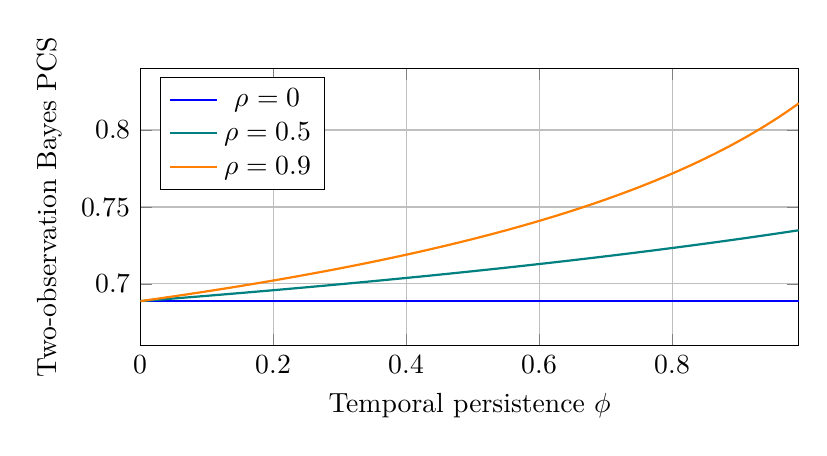
\begin{tikzpicture}
\begin{axis}[width=.82\textwidth,height=5.1cm,xlabel={Temporal persistence $\phi$},ylabel={Two-observation Bayes PCS},xmin=0,xmax=.99,ymin=.66,ymax=.84,legend pos=north west,grid=major]
\addplot[blue,thick,domain=0:.99,samples=80]{.5+atan(1/sqrt(2*(1+.1)))/180};
\addlegendentry{$\rho=0$}
\addplot[teal,thick,domain=0:.99,samples=80]{.5+atan(1/sqrt(2*(1-.5*x+.1)))/180};
\addlegendentry{$\rho=0.5$}
\addplot[orange,thick,domain=0:.99,samples=80]{.5+atan(1/sqrt(2*(1-.9*x+.1)))/180};
\addlegendentry{$\rho=0.9$}
\end{axis}
\end{tikzpicture}
\caption{Exact two-observation permanent-mean PCS at $V=1$, $r=0.1$, $\alpha=1$, and $\lambda w=0.5$. Positive cross-location persistence helps a paired contrast. This is not a general monotonicity claim for longer-horizon learning or a fixed-gap comparison across different mean priors.}
\label{fig:two-pcs}
\end{figure}

\section{Graph modes and the cost of temporal redundancy}
\begin{proposition}[Full-field benchmark]
Suppose all locations are observed exactly at each of $n$ consecutive times, with $r=0$. This is a stronger feedback benchmark costing $Nn$ scalar measurements. Then
\begin{equation}
\mathcal I_n=a_nK_z^{-1},\qquad
\boxed{a_n=\frac{n(1-\phi)+2\phi}{1+\phi}.}
\label{eq:full-field-info}
\end{equation}
If $K_z=U\operatorname{diag}(k_j)U^\top$ shares the Laplacian eigensystem, posterior graph-mode variances are
\begin{equation}
\boxed{s_j^2=\{a_n/k_j+\alpha+\lambda\ell_j\}^{-1}.}
\label{eq:mode-posterior}
\end{equation}
For unanchored Laplacian ridge ($\alpha=0$), with $\theta_j=(U^\top\mu)_j$, mode MSE is
\begin{equation}
\left(\frac{\lambda\ell_j}{a_n/k_j+\lambda\ell_j}\right)^2\theta_j^2
+\frac{a_n/k_j}{(a_n/k_j+\lambda\ell_j)^2}.
\label{eq:mode-risk}
\end{equation}
\end{proposition}
\begin{proof}
The full observation covariance is $R_n(\phi)\otimes K_z$ and its mean design is $\one_n\otimes I$. Thus information is $(\one_n^\top R_n^{-1}\one_n)K_z^{-1}$. The tridiagonal inverse AR correlation matrix gives~\eqref{eq:full-field-info}, including $a_1=1$. Simultaneous diagonalization gives~\eqref{eq:mode-posterior} and the fixed-design bias/variance formula gives~\eqref{eq:mode-risk}.
\end{proof}

For $\phi\uparrow1$ with fixed $n$ and fixed stationary variance, $a_n\to1$: a nearly constant transient field is difficult to distinguish from a permanent mean. For fixed $\phi<1$ and large $n$, information grows at rate $(1-\phi)/(1+\phi)$. Good short-term prediction can coexist with slow permanent-mean estimation. At the excluded boundary $\phi=1$, repeated noiseless observation of $\mu+z_1$ does not separately identify the two components.

Pairwise posterior variance is
\begin{equation}
\Var(\mu_i-\mu_j\mid Y)=\sum_k(U_{ik}-U_{jk})^2s_k^2.
\end{equation}
The constant graph mode cancels. Spatial smoothness is meaningful for selection when it constrains modes distinguishing competing locations, rather than merely reducing uncertainty about a global level.

When $\phi=0$ and only one coordinate is observed per calendar round, off-diagonal entries of $K_z$ disappear from~\eqref{eq:xi}. If its diagonal is fixed, $\mathcal I$ is simply the diagonal count matrix divided by the marginal observation variance. The permanent mean graph can still help through $H$; transient spatial correlation contributes no cross-time mean information in this control case.

\section{Information limits and the distinction from tracking regret}
For a fixed design, any two deterministic means have likelihood divergence
\begin{equation}
\KL(P_\mu,P_\nu)=\tfrac12(\mu-\nu)^\top\mathcal I_T(\mu-\nu).
\end{equation}
For a non-anticipating policy with finite horizon, chain rule and~\eqref{eq:regression} instead give
\begin{equation}
\boxed{\KL(P_\mu^{\pi,T},P_\nu^{\pi,T})
=\tfrac12\E_\mu[(\mu-\nu)^\top\mathcal I_T(\mu-\nu)].}
\label{eq:adaptive-kl}
\end{equation}
The action probabilities cancel, and each conditional Gaussian divergence equals $(u_t^\top(\mu-\nu))^2/2$. If a recommendation is $\delta$-correct at both means and their unique best arms differ, data processing gives the necessary condition
\begin{equation}
\tfrac12\E_\mu[(\mu-\nu)^\top\mathcal I_T(\mu-\nu)]
\ge\operatorname{kl}(1-\delta,\delta),\qquad \delta<1/2.
\end{equation}
Restricting $\nu$ to a valid graph-energy class connects correctness of the mean graph to exploration requirements. This is a specialization of established change-of-measure reasoning~\cite{combes2017,garivier2016}; counts alone cannot generally replace the adaptive information matrix. No algorithm is proved to attain this instance-specific information program here.

For ongoing reward, a full-current-state oracle can choose $\argmax_i f_{i,t}$, whereas a causal learner acts before observing the current field. With known $\mu$, define $G(\mu,C)=\E\max_i(\mu_i+Z_i)$ for $Z\sim N(0,C)$. A genie seeing every past state predicts the current residual with covariance $\phi^2K_z$ and still lacks fresh innovations. Consequently
\begin{equation}
R_T^\pi\ge T\{G(\mu,K_z)-G(\mu,\phi^2K_z)\}.
\end{equation}
The bound follows from the genie's maximum conditional mean and convexity of the maximum. It is positive for nondegenerate contrast innovations. It does not prevent consistent permanent-mean selection, whose error can vanish under forced coverage. These two objectives require different benchmarks.

\section{Reproducible experiments}
The primary experiment uses six nodes on an unweighted path. The permanent means are drawn once from
\[
\mu\sim N\{0,(I+\lambda_{\rm true}L)^{-1}\},\qquad
\lambda_{\rm true}\in\{0,2\}.
\]
Residual covariance is a diagonally normalized resolvent $(I+2L)^{-1}$, with marginal residual variances one; measurement variance is $0.1$. Persistence is $0$, $0.9$, or $0.99$. Every configuration uses 200 independent paired trajectories and 48 sequential measurements. Within a trajectory all policies share the same means, latent field, and potential measurement noises. The normalized residual covariance need not commute with the raw path Laplacian; the full-field spectral formulas assume commuting covariances explicitly and are not imposed on this experiment.

Seven specified policies are compared. Graph--AR KG uses the fitted mean prior $(I+2L)^{-1}$ and correct AR likelihood. Unstructured--AR KG uses mean prior $I$, matching the rough-mean generative case. Diagonal-mean--AR KG retains the fitted graph prior's marginal variances but removes its cross-covariances. Graph--iid KG uses the graph mean prior but incorrectly assumes $\phi=0$ when persistence is positive. Wrong-mean-graph--AR KG permutes the mean graph while retaining the correct residual dynamics. The contrast rule uses~\eqref{eq:contrast-gain}. Round robin uses the graph--AR posterior with a fixed cyclic design. Non-round-robin policies force a cyclic location once every seven measurements, ensuring eventual coverage.

Every policy recommends the largest posterior mean, so the reported PCS is the accuracy of that recommendation and is not a general Bayes-PCS optimum. The main sampling objective is opportunity loss. We also report mean-estimation MSE and coverage of a fixed endpoint contrast by a 95\% posterior interval. Such coverage has a Bayesian interpretation only for the matched model. The separate all-time frequentist audit tests graph--AR KG and supplies each sampled truth's actual norm and graph energy as valid radii; policies do not use those radii. This audits a conditional theorem under trusted certificates, not a method for obtaining them. Its per-configuration coverage is repeated in the CSV rows and is not an audit of misspecified filters.

\begin{table}[p]
\centering\small
\begin{tabular}{rrlrrr}
\toprule
$\lambda_{\rm true}$ & $\phi$ & Policy & EOC & PCS & MSE \\
\midrule
0 & 0 & Graph--AR KG & 0.042 & 0.765 & 0.309 \\
0 & 0 & Unstructured--AR KG & 0.038 & 0.805 & 0.151 \\
0 & 0 & Graph--iid KG & 0.044 & 0.780 & 0.301 \\
0 & 0 & Round robin & 0.104 & 0.720 & 0.217 \\
0 & 0.9 & Graph--AR KG & 0.099 & 0.730 & 0.364 \\
0 & 0.9 & Unstructured--AR KG & 0.104 & 0.710 & 0.245 \\
0 & 0.9 & Graph--iid KG & 0.162 & 0.625 & 0.440 \\
0 & 0.9 & Round robin & 0.114 & 0.700 & 0.296 \\
0 & 0.99 & Graph--AR KG & 0.292 & 0.570 & 0.583 \\
0 & 0.99 & Unstructured--AR KG & 0.253 & 0.605 & 0.422 \\
0 & 0.99 & Graph--iid KG & 0.288 & 0.570 & 0.718 \\
0 & 0.99 & Round robin & 0.322 & 0.545 & 0.573 \\
2 & 0 & Graph--AR KG & 0.067 & 0.735 & 0.107 \\
2 & 0 & Unstructured--AR KG & 0.084 & 0.680 & 0.132 \\
2 & 0 & Graph--iid KG & 0.072 & 0.725 & 0.106 \\
2 & 0 & Round robin & 0.088 & 0.655 & 0.093 \\
2 & 0.9 & Graph--AR KG & 0.191 & 0.500 & 0.198 \\
2 & 0.9 & Unstructured--AR KG & 0.210 & 0.500 & 0.244 \\
2 & 0.9 & Graph--iid KG & 0.205 & 0.530 & 0.279 \\
2 & 0.9 & Round robin & 0.174 & 0.520 & 0.181 \\
2 & 0.99 & Graph--AR KG & 0.274 & 0.385 & 0.253 \\
2 & 0.99 & Unstructured--AR KG & 0.247 & 0.420 & 0.318 \\
2 & 0.99 & Graph--iid KG & 0.293 & 0.405 & 0.519 \\
2 & 0.99 & Round robin & 0.286 & 0.390 & 0.251 \\
\bottomrule
\end{tabular}

\caption{Permanent-mean experiment: expected opportunity cost (EOC), PCS of the largest-posterior-mean recommendation, and MSE per mean. Each entry uses 200 paired runs, budget 48, and six locations. Standard errors, variance-matched diagonal-prior comparisons, wrong-graph comparisons, coverage, and paired uncertainty are supplied in the accompanying CSVs and findings.}
\label{tab:experiment}
\end{table}

For matched smooth means, graph--AR KG MSE is approximately $0.107$, $0.198$, and $0.253$ as persistence increases. The graph--iid model gives approximately $0.106$, $0.279$, and $0.519$, with endpoint contrast coverage falling to $0.62$ at persistence $0.99$. The diagonal-mean baseline gives MSE approximately $0.121$, $0.230$, and $0.270$, isolating removal of prior correlation while retaining its marginal variances. These finite examples support covariance-aware estimation; they do not establish uniform superiority of the KG policy.

The policy comparison also exposes limitations. At matched smooth means and $\phi=0.9$, round robin has opportunity loss about $0.174$, versus $0.191$ for graph--AR KG. At $\phi=0.99$, unstructured--AR KG gives about $0.247$ versus $0.274$ for graph--AR KG. The paired intervals are reported rather than treating every mean difference as conclusive. At rough means and $\phi=0$, graph--AR KG MSE is about $0.309$ versus $0.151$ for the matching unstructured prior, and its endpoint contrast coverage is $0.85$. An incorrect smooth prior can distort permanent-mean estimates even when the AR likelihood is correct.

Exact calculations are checked independently of the policy experiment. Online information, scores, and posterior updates agree with dense trajectory likelihood calculations across positive, zero, and negative persistence. Constrained estimation enforces its supplied energy; fixed-design contrast bias matches the algebra. A broad two-location grid, including negative spatial correlation, validates the two-observation closed forms and design ordering. Three independent prior-predictive checks use 50,000 draws each; observed PCS agrees with the closed form within Monte Carlo uncertainty. A zero-persistence control verifies removal of transient cross-location information. The full-field effective sample-size identity is checked using independent dense solves. The current script passes 8,888 counted assertions; these are numerical checks, not a substitute for the proofs.

The standard-library script is \path{experiments/simulations/theory/spatiotemporal/graph_ar1_mean.py}. Accompanying data are in this manuscript's \path{results/mean_selection/} directory. The initial known-zero-mean reward experiment is retained separately and is not evidence for the permanent-mean estimates in this manuscript.

\section{Discussion and research agenda}
The tractable model gives a direct answer to how spatial smoothness should be used. Fit means using the actual covariance of the observed trajectory, regularize differences on the graph, and retain the resulting bias or prior uncertainty. In a frequentist formulation, meaningful smoothing requires a trusted quantitative radius; in a Bayesian formulation, it requires a defensible prior. Neither smoothing a graph nor a small posterior variance verifies that assumption from selected-arm data.

The formulation differs from a pure time-varying GP tracking problem through its permanent target, from iid graph pure exploration through its colored observation likelihood, and from classical correlated-normal KG through its history-dependent whitened experiments. These distinctions motivate specialized results, but the overall model remains within established GP and linear Gaussian families.

A stronger publication contribution would characterize the optimal schedule-dependent information for graph-constrained alternatives, develop an allocation attaining it, and quantify restricted graph and temporal misspecification under adaptive feedback. The stopping rule here is correct with supplied certificates but has conservative sample bounds. Rolling KG is computable but can lose to fixed allocation. Extending to unknown covariance, seasonality, varying costs, and actual profit targets requires additional assumptions and validation.

\appendix
\section{Implementation and interpretation details}
The two filters maintained in innovation regression are not an independence approximation between mean and noise. The state $(g,D,P)$ describes the conditional noise distribution at a fixed candidate mean. The posterior $(M,S)$ integrates that affine dependence exactly. For example, the next reward predictor at node $i$ is $g_i+(e_i+D_i)^\top M$, and its latent variance is
\[
P_{ii}+(e_i+D_i)^\top S(e_i+D_i).
\]
The mean-target measurement covariance is $Sv_{t,a}$ and its total predictive observation variance is $d_{t,a}+v_{t,a}^\top Sv_{t,a}$. Thus the target slopes used by KG equal $Sv_{t,a}/\sqrt{d_{t,a}+v_{t,a}^\top Sv_{t,a}}$, which agrees with~\eqref{eq:kg}.

The batch likelihood at a completed adaptive history is evaluated at its recorded node-time pairs. Its Gaussian form in the unknown mean is legitimate because policy probabilities add no parameter-dependent factor once the recorded observations are fixed. Nevertheless, repeated-sampling distributions conditional on those random node-time pairs can be distorted. The adaptive martingale confidence and~\eqref{eq:adaptive-kl} explicitly avoid that conditioning error.

Stronger mean smoothness shrinks prior difference variances. Comparing Bayesian PCS across different mean priors changes both inference and the distribution of true gaps; monotonic posterior variance does not imply monotonic PCS. The two-location MSE/PCS distinction and the finite-horizon experiment are intended to prevent this interpretation error.

Reproduce from the repository root:
\begin{verbatim}
python3 experiments/simulations/theory/spatiotemporal/graph_ar1_mean.py --verify
python3 experiments/simulations/theory/spatiotemporal/graph_ar1_mean.py --runs 200 --budget 48
python3 experiments/simulations/theory/spatiotemporal/graph_ar1_mean.py --render-only
cd research/spatiotemporal_bandits
tectonic --only-cached --keep-logs manuscript.tex
\end{verbatim}

\begin{thebibliography}{99}
\raggedright
\bibitem{valko2014} M. Valko, R. Munos, B. Kveton, and T. Koc\'{a}k. Spectral Bandits for Smooth Graph Functions. ICML, PMLR 32(2):46--54, 2014. \url{https://proceedings.mlr.press/v32/valko14.html}.
\bibitem{thaker2022} P. Thaker, M. Malu, N. Rao, and G. Dasarathy. Maximizing and Satisficing in Multi-armed Bandits with Graph Information. NeurIPS 35, 2022. \url{https://papers.neurips.cc/paper_files/paper/2022/hash/0d561979f0f4bc6127cfcfe9c46ee205-Abstract-Conference.html}.
\bibitem{bogunovic2016} I. Bogunovic, J. Scarlett, and V. Cevher. Time-Varying Gaussian Process Bandit Optimization. AISTATS, PMLR 51:314--323, 2016. \url{https://proceedings.mlr.press/v51/bogunovic16.html}.
\bibitem{krause2011} A. Krause and C. S. Ong. Contextual Gaussian Process Bandit Optimization. NIPS 24, 2011. \url{https://papers.nips.cc/paper/2011/hash/f3f1b7fc5a8779a9e618e1f23a7b7860-Abstract.html}.
\bibitem{gornet2024} J. Gornet and B. Sinopoli. Restless bandits with rewards generated by a linear Gaussian dynamical system. L4DC, PMLR 242:1791--1802, 2024. \url{https://proceedings.mlr.press/v242/gornet24a.html}.
\bibitem{trella2025} A. L. Trella, W. H. Dempsey, A. Gazi, Z. Xu, F. Doshi-Velez, and S. Murphy. Non-Stationary Latent Auto-Regressive Bandits. Reinforcement Learning Journal 6:765--789, 2025. \url{https://rlj.cs.umass.edu/2025/papers/Paper70.html}.
\bibitem{frazier2009} P. Frazier, W. B. Powell, and S. Dayanik. The Knowledge-Gradient Policy for Correlated Normal Beliefs. INFORMS Journal on Computing 21(4):599--613, 2009. \url{https://doi.org/10.1287/ijoc.1080.0314}.
\bibitem{abbasi2011} Y. Abbasi-Yadkori, D. P\'{a}l, and C. Szepesv\'{a}ri. Online Least Squares Estimation with Self-Normalized Processes: An Application to Bandit Problems. 2011 preprint. \url{https://arxiv.org/abs/1102.2670}.
\bibitem{combes2017} R. Combes, S. Magureanu, and A. Proutiere. Minimal Exploration in Structured Stochastic Bandits. NIPS 30, 2017. \url{https://papers.nips.cc/paper_files/paper/2017/hash/e19347e1c3ca0c0b97de5fb3b690855a-Abstract.html}.
\bibitem{garivier2016} A. Garivier and E. Kaufmann. Optimal Best Arm Identification with Fixed Confidence. COLT, PMLR 49:998--1027, 2016. \url{https://proceedings.mlr.press/v49/garivier16a.html}.
\bibitem{ziomek2025} J. Ziomek, M. Adachi, and M. A. Osborne. Time-varying Gaussian Process Bandits with Unknown Prior. AISTATS, PMLR 258:4294--4302, 2025. \url{https://proceedings.mlr.press/v258/ziomek25a.html}.
\bibitem{guneyi2024} E. T. G\"uneyi, B. Yald\i z, A. Canbolat, and E. Vural. Learning Graph ARMA Processes From Time-Vertex Spectra. IEEE Transactions on Signal Processing 72:47--56, 2024; online publication November 2023. \url{https://doi.org/10.1109/TSP.2023.3329948}.
\end{thebibliography}
\end{document}
